
\section{The ICA Problem}
\begin{frame}{\secname}

independent sources: $\vec s = (s_1, s_2,...,s_N)^\top \in \R^N$\\
observations: $\vec x \in \R^N$

\begin{equation}
\label{eq:ica}
\vec x = \vec A \, \vec s
\end{equation}

\begin{equation}
\widehat{\vec s} = \vec W \vec x
\end{equation}

Methods for solving the ICA problem:

\begin{itemize}
\item maximizing the \emph{mutual information} between $\vec x$ and $\vec {\hat s}$ \\
(e.g. Infomax)
\item maximizing the \emph{nongaussianity} of $\widehat {\vec s}$ \\
(e.g. Kurtosis-based ICA, FastICA)
\end{itemize}
\end{frame}

\begin{frame}
\underline{Outline:}
\begin{itemize}
    \item ICA on whitened data
    \begin{itemize}
        \item Whitening/sphering
        \item Amibguities in ICA
        \item PCA is \emph{half} the ICA Problem
    \end{itemize}
    \item the problem with gaussians
    \item maximizing nongaussianity
    \begin{itemize}
        \item Kurtosis-based
        \item negentropy
    \end{itemize}
\end{itemize}
\end{frame}

\newpage

\section{Whitening revisited}

\begin{frame}{\secname}

\notesonly{
The purpose of whitening is to decorrelate the data.
}

Let the data $\vec X \in \R^{N \times p}$ be centered:

\begin{equation}
\label{eq:centered}
\E \lbrack \vec x \rbrack = 0 
\end{equation}

\notesonly{
From this follows:
}

\begin{equation}
\label{eq:cov}
\vec \Sigma_x = \mathrm{Cov}(\vec x) = \E \lbrack \, \vec x \, \vec x^\top \rbrack 
\end{equation}

The whitening transformation yields:

\begin{equation}
\label{eq:whitening}
\vec v^{(\alpha)} = \vec \Lambda^{-\frac{1}{2}} \vec M^\top \vec x^{(\alpha)}
\end{equation}

where
\begin{itemize}
\item[] $\vec M = (\vec e_1, \vec e_2, \ldots,\vec e_N)$ is the orthonormal eigenbasis of $\Sigma_x$
\item[] and $\vec\Lambda$ is diagonal matrix with the corresponding eigenvalues.
\end{itemize}

\pause

\question{What do we know about the variables in $\vec v$?}

\pause

\begin{equation}
\label{eq:covw}
\vec \Sigma_v = \mathrm{Cov}(\vec v) = \E \lbrack \, \vec v \, \vec v^\top \rbrack = \vec I_N
\end{equation}

\notesonly{
Uncorrelated means zero covariance. Therefore, the covariance matrix for uncorrelated data is a diagonal matrix because it only contains the variances of the individual variables. 
Whitening decorrelates the variables and normalizes the variances to 1.
}
\end{frame}

\begin{frame}{\secname}

\begin{figure}[ht]
\label{fig:sphering}
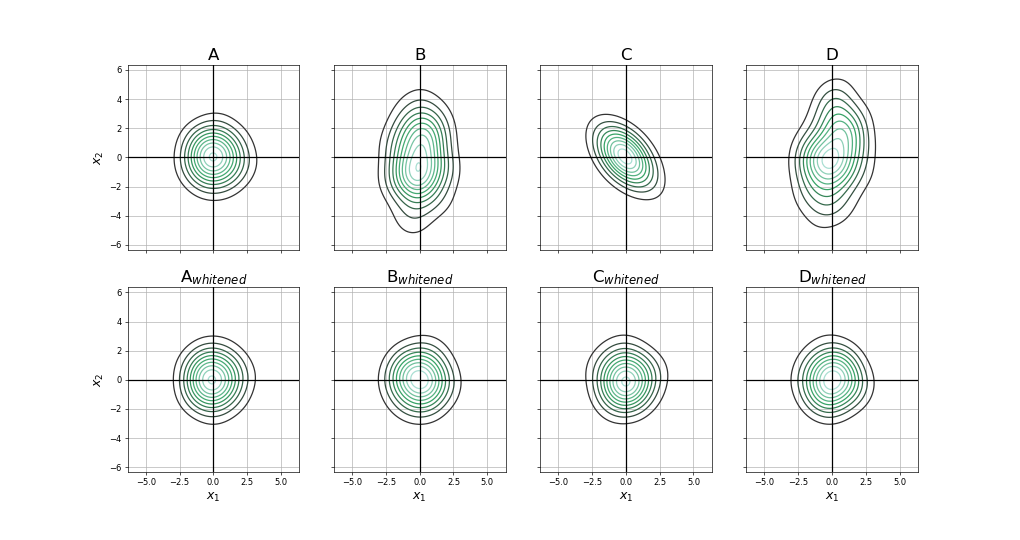
\includegraphics[width=12cm]{img/cov.png}
\caption{A visual interpretation of whitening}
\end{figure}

\end{frame}
